%% ****** Start of file aiptemplate.tex ****** %
%%
%%   This file is part of the files in the distribution of AIP substyles for REVTeX4.
%%   Version 4.2 of December 2014.
%%
%
% This is a template for producing documents for use with 
% the REVTEX 4.2 document class and the AIP substyles.
% 
% Copy this file to another name and then work on that file.
% That way, you always have this original template file to use.

\documentclass[aip,reprint]{revtex4-2}
%\documentclass[aip,reprint]{revtex4-2}

\usepackage{graphicx}% Include figure files
\usepackage{dcolumn}% Align table columns on decimal point
\usepackage{bm}% bold math
\usepackage{amsmath}
\usepackage{amssymb}
\usepackage{caption, subcaption}
\usepackage{usual}
\usepackage{array}

\draft % marks overfull lines with a black rule on the right

\begin{document}

% Use the \preprint command to place your local institutional report number 
% on the title page in preprint mode.
% Multiple \preprint commands are allowed.
%\preprint{}

\title[Pump coupling optimizied 3-wave-mixing Josephson parametric amplifier]{Pump coupling optimizied 3-wave-mixing Josephson parametric amplifier} %Title of paper

% repeat the \author .. \affiliation  etc. as needed
% \email, \thanks, \homepage, \altaffiliation all apply to the current author.
% Explanatory text should go in the []'s, 
% actual e-mail address or url should go in the {}'s for \email and \homepage.
% Please use the appropriate macro for the type of information

% \affiliation command applies to all authors since the last \affiliation command. 
% The \affiliation command should follow the other information.

\author{(authors)}
%\email[]{Your e-mail address}
%\homepage[]{Your web page}
%\thanks{}
%\altaffiliation{}
\affiliation{Department of Applied Physics, Yale University, New Haven, CT 06520, USA}

% Collaboration name, if desired (requires use of superscriptaddress option in \documentclass). 
% \noaffiliation is required (may also be used with the \author command).
%\collaboration{}
%\noaffiliation

\date{\today}

\begin{abstract}

Three-wave mixing Josephson parametric amplifiers (JPAs) typically require pump that is 6 to 7 orders of magnitude stronger than the signal power it can handle. The leakage of pump towards signal circuitry is generally harmful in application. We would also like to bring power efficiency, defined as the ratio between maximum output power in linear amplification regime and pump power required, into future concern of the JPA community. We propose a JPA that minimizes pump leakage and at the same time maximizes the pump coupling efficiency. By applying on-chip microwave filtering on a 3-wave-mixing JPA whose pump is off-resonance, we engineer dual-band coupling networks which satisfy different conditions at signal frequency and pump frequency separately. We show experimentally that more than 20dB improvement in power efficiency and more than 20dB suppression of pump leakage can be achieved by the filtering technique, while maintaining dynamic range and near-quantum limited noise performance. 

\end{abstract}

\maketitle %\maketitle must follow title, authors, abstract

% Body of paper goes here. Use proper sectioning commands. 
% References should be done using the \cite, \ref, and \label commands
\section{Introduction}

(General background)
\begin{itemize}
	\item (In JPA applications, minimum backaction is usually wanted)
	\item JPAs require strong pump to work
	\item Pump leakage are bad and need to be dealt with
	\item Geneneally, the higher power handling ability a JPA has, the stronger pump it requires: 
	\begin{enumerate}
		\item Might require extra efforts on pump isolation
		\item Concerning fridge cooling power, the pump power we can deliver could become a limiting factor
	\end{enumerate}
\end{itemize}

Josephson parametric amplifiers (JPAs) are commonly used in precision microwave measurements, such as superconducting qubit readout, microwave optomechanics experiment, electron spin resonance measurement, and Axion detection. Besides low added noise, usually minimum backaction is also wanted in such applications. All JPAs require rf pump that is orders of magnitude stronger than input signal. If not dealt with properly, JPA pump could harm the \textbf{system under measurement}. Usually external non-reciprocal components are employed to achieve directionality, as well as isolating the \textbf{system under measurement} from pump in amplifier circuitry. 

% Minimizing this pump leakage from signal port is wanted for qubit protection, yet no previous work has made any optimization in this direction. 

Many recent researches are focused on improving dynamic range of JPAs. While JPAs with higher signal power handling ability generally need higher pump power, which might need extra efforts on pump isolation. In addition, concerning cooling power of dilution fridges, the maximum pump power we can deliver at the JPA could itself become a limiting factor. 

(Detailed background about 3wm JPAs)

\begin{itemize}
	\item Pump that is close to signal frequency is usually more harmful
	\item Compared to 4wm JPAs, 3wm JPAs has the advantage that they're pumped off-resonance
	\item However, pump being off-resonance makes it poorly coupled
	\item As a result, 3wm JPAs typically require larger pump power delivered (than 4wm JPAs) to work
\end{itemize}


Resonance JPAs amplifies signal that is close to its resonance frequency $\omega_a$. Therefore, presence of on-resonance pump is usually more harmful, for the \textbf{systems under measurement} are typically more susceptible to noise near signal frequency. In this sense, the fact that a 3-wave-mixing JPA is pumped off-resonance is advantageous over 4-wave-mixing JPAs whose pump is on-resonance. 

However, pump being detuned from the amplifier mode typically makes the pump poorly coupled to 3-wave-mixing JPAs. As a result, in order to achieve sufficient intra-device pump strenth to work, more pump power need to be delivered at 3-wave-mixing JPAs compared to that required for 4-wave-mixing JPAs. \\


(Intro of this paper)
\begin{itemize}
	\item Propose a technique (filtering) that applies to 3wm JPAs to:
	\begin{enumerate}
		\item Suppress pump leakage
		\item Enable efficient pumping
	\end{enumerate}
	\item From experimental comparison between a common two-port SPA and a \textbf{filter coupled SPA}, we show that the latter:  
	\begin{enumerate}
		\item Shows **dBm less pump leakage from signal port at 20dB gain working condition
		\item Require **dBm less pump power delivered at pump port to achieve \textbf{20dB low signal gain}
	\end{enumerate}
\end{itemize}


\begin{figure*}[htb]
\subcaptionbox{capacitively coupled SPA}
{\label{fig:device1}
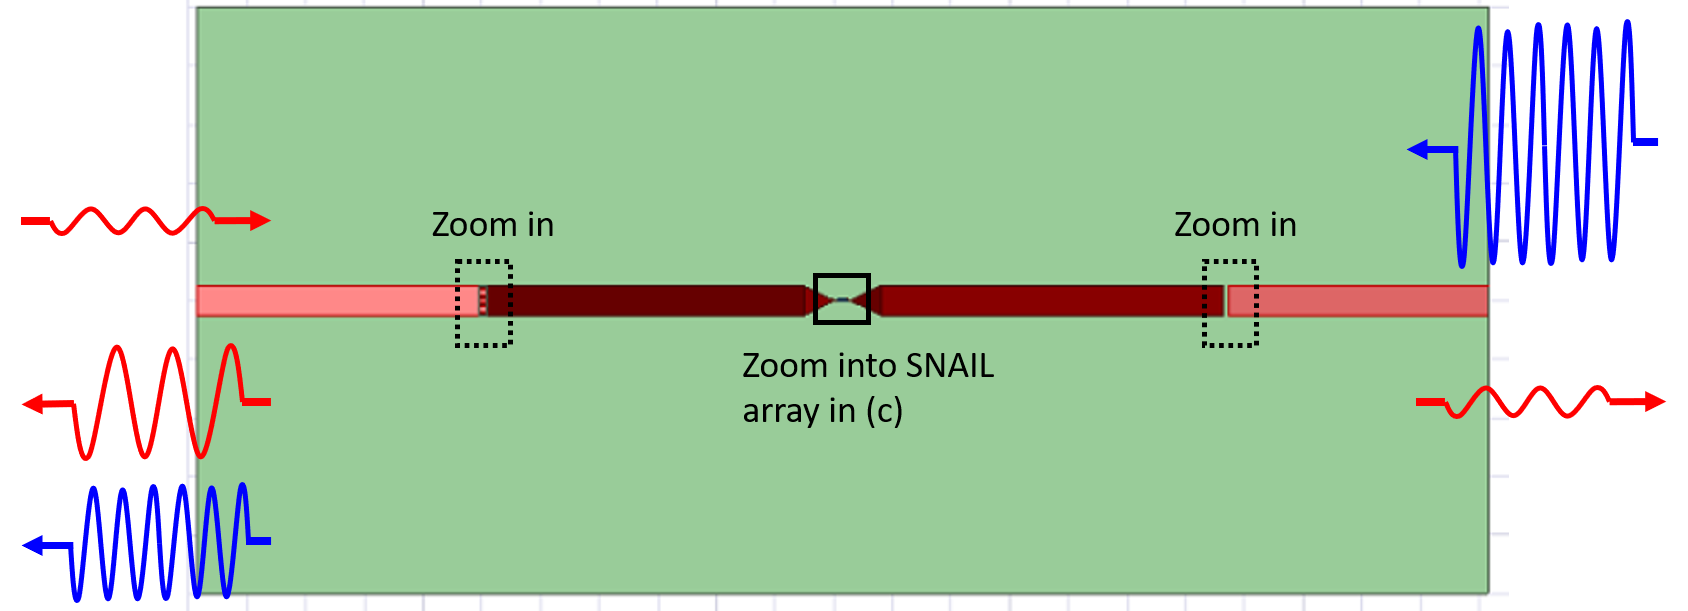
\includegraphics[width=8.5cm]{figures/SPA.PNG}
}
\subcaptionbox{filter coupled SPA}
{\label{fig:device2}
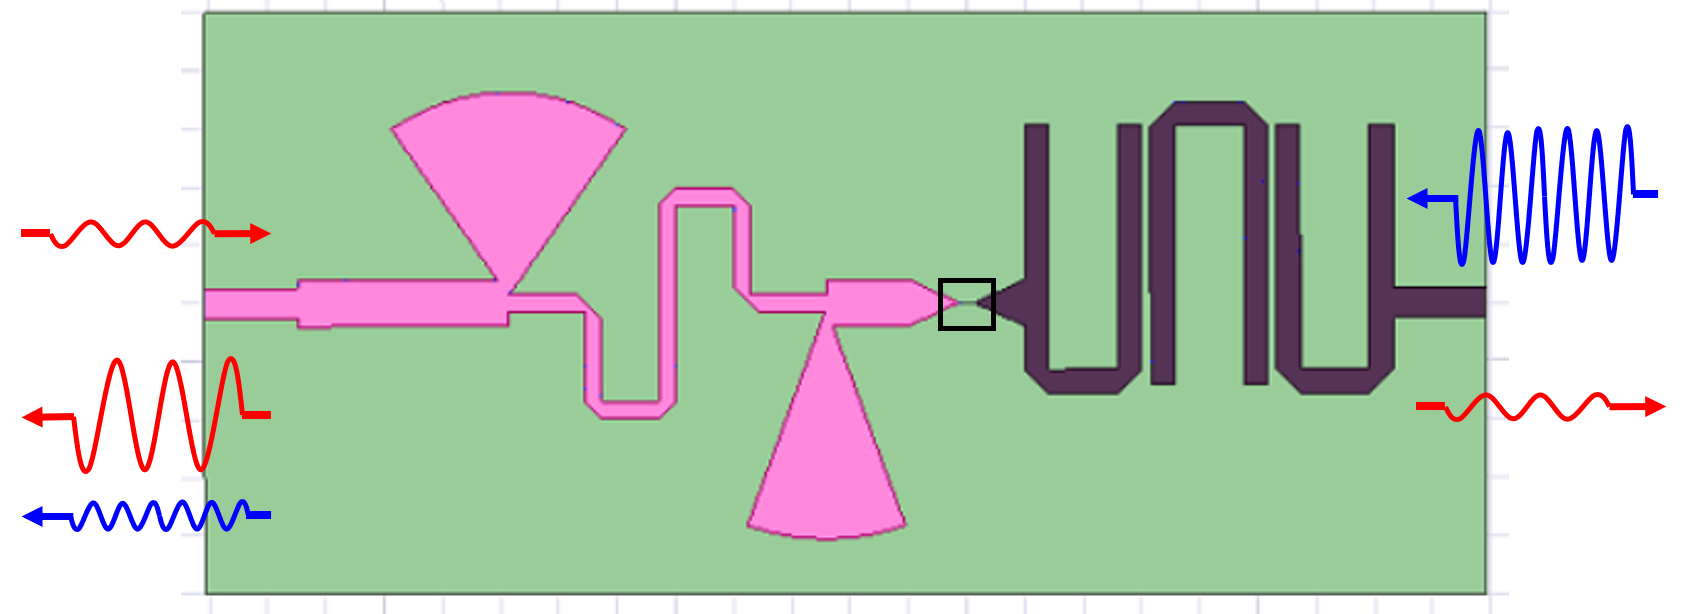
\includegraphics[width=8.5cm]{figures/FSPA.PNG}
}
\subcaptionbox{General circuit model: SPA with arbitrary linear network at both ports}
{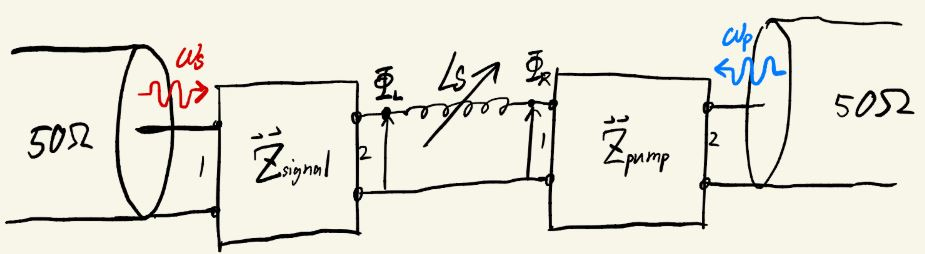
\includegraphics[width=15cm]{figures/circuit_1}
\label{fig:circuit_1} 
}
\caption
{\label{fig:device} Layout of a capacitively coupled SPA and a filter coupled SPA. Reflection gain is obtained from signal port, and minimal signal leakage from pump port is expected. Originally, different coupling capacitors are employed at signal and pump port. We suggest that a bandstop filter (pink) at signal port can suppress pump leakage while maintaining moderate signal coupling. And a bandpass filter (purple) at pump port provide strong coupling for pump and weak coupling for signal. }
\end{figure*}


In this letter, we demonstrate a technique that applies to 3-wave-mixing JPAs to suppress pump leakage towards qubit as well as enable efficient pumping. We present a 3-wave-mixing JPA that has two rf ports with on-chip microwave filtering. One port, which is referred to as “signal port”, provides reflection gain for input signal. The other port which I name “pump port” is for current pumping. We have shown that, compared to a similar device with traditional capacitively coupled ports\cite{SPA,Kerr_free}, \textbf{the filter coupled SPA} 1) shows 20dB less pump leakage from signal port, and 2) requires 20dB less pump power delivered at device pump port, when achieving the same amplification condition. 

% \begin{figure*}
% \subcaptionbox{one-port JPA}
% {
% 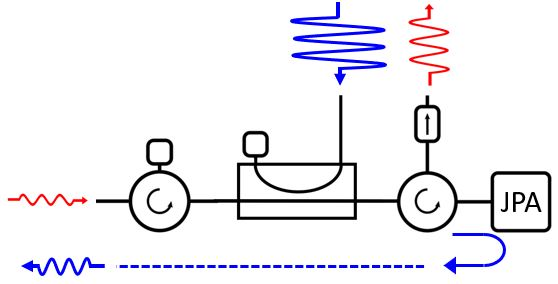
\includegraphics[height=4cm]{figures/one-port.JPG}
% }
% \subcaptionbox{two-port JPA}
% {
% 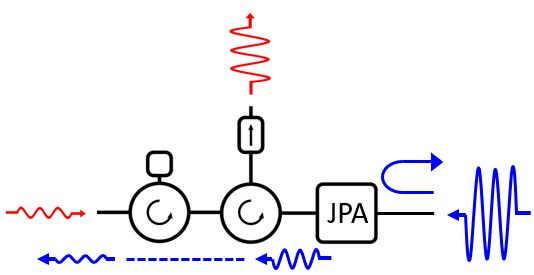
\includegraphics[height=4.2cm]{figures/two-port.JPG}
% }
% \caption
% {\label{fig:diagram} (Diagram illustrating how pump is applied to one-port JPA and two-port JPA)}
% \end{figure*}

\section{Introduce device}

\begin{itemize}
	\item SPA: a degenerate JPA based on 3wm nonlinearity from SNAIL participation
	\item Having a separate pump port is favorable for qubit protection
	\item $\kappa^{(p)}[\omega_s]$ has to be small for noise property
	\item Pump power required to achieve 20dB gain: 
	\begin{enumerate}
		\item Gain depends on $\alpha_p$
		\item $\alpha_p$ depends on pump power and pump port coupling $\kappa^{(p)}[\omega_p]$
	\end{enumerate}
	\item $\kappa^{(s)}[\omega_s]$ has to guarantee moderate bandwidth
	\item $\kappa^{(s)}[\omega_p]$ and $\alpha_p$ determines pump leakage
	\item Frequency separation between signal and pump allows for engineering different $\kappa[\omega_s]$ and $\kappa[\omega_p]$ 
\end{itemize}


The device in this work is a SNAIL parametric amplifier (SPA)\cite{SPA}, by which we refer to a degenerate parametric amplifier formed by a resonance mode with Superconducting Nonlinear Asymmetric Inductive eLement (SNAIL)\cite{SNAIL} participation. 


A traditional SPA \cite{SPA,Kerr_free} is formed by an array of SNAILs sitting at the center of a $\lambda/2$ microstrip resonantor, as shown in \fig{fig:device} (a). An SPA has Hamiltonian with third and fourth order nonlinearity: 

\begin{equation}\label{eq:H_SPA}
H_\mathrm{SPA} = \hbar \omega_a \ad a + g_3 (\ad + a)^3 + g_4 (\ad + a)^4
\end{equation}

Upon pumping at frequency $\omega_p \approx 2\omega_a$, Quantum Langevin Equation (QLE) gives phase preserving power gain: 

\begin{equation}\label{eq:G}
G = 1 + \frac{4\kappa^2 \abs{g}^2}{\(\Delta^2 + \frac{\kappa^2}{2} - 4\abs{g}^2\)^2}
\end{equation}
for signal frequency $\omega_s \approx \omega_p/2$ and low signal power, where $g = 2 g_3 \alpha_p$ with $\alpha_p$ being mean-field intra-device pump amplitude, and $\Delta = \omega_a + \( \frac{32}{3}g_4 - 28\frac{g_3^2}{\omega_a} \) \abs{\alpha_p}^2 - \frac{\omega_p}{2} $ is detuning between $\omega_p/2$ and Stark-shifted mode frequency due to $\alpha_p$. 




% An SPA, or generally a resonance JPA, do not necessarily need a separate port for current pumping. 
Although it's possible to apply current pumping from the same port as signal, having a separate port for pump is favored as it removed the necessity of directional couplers or multiplexers in front of signal port. And more importantly, reflected power due to pump port mismatch doesn’t see the qubit circuitry, which greatly eases pump isolation. 

In this case, signal leakage from pump port has to be minimized to guarantee near-quantum-limited noise performance. Thus the pump port in \fig{fig:device} (a) is weakly coupled which, on the other hand, makes pump coupling rate badly low and worsens the pump power inefficiency problem of 3-wave-mixing JPAs. 

Signal port coupling capacitor is typically made to achieve coupling rate $\kappa/2\pi$ on the order of 100 MHz. While intra-mode pump also leaks into signal line via this coupling capacitor, yet no previous work has been focused on reducing pump leakage. 

Pump leakage due to signal port coupling and pump inefficiency due to pump port coupling can be addressed with the same idea of microwave filtering. The frequency separation between signal and pump in 3-wave-mixing JPAs can be utilized, enabling significantly different coupling rate at $\omega_s$ and $\omega_p$. 

\begin{figure}[htb]
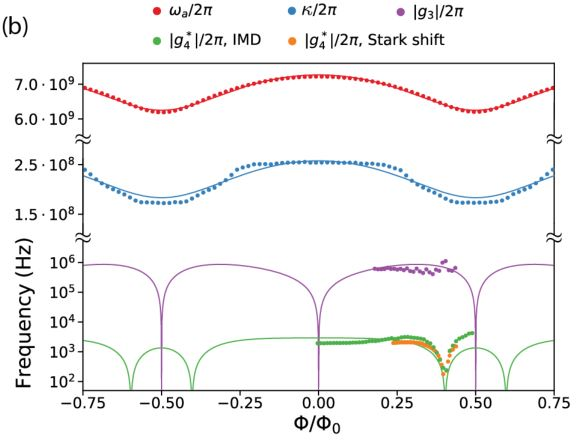
\includegraphics[width=6.5cm]{figures/FluxSweep.jpg}
\caption
{\label{fig:flux_sweep} Flux sweep showing frequency, kappa, g3 and g4 (this is from Vlad's paper)}
\end{figure}






\section{Model}

\begin{itemize}
	\item A resonance mode at $\omega_a$ with SNAIL participation has to be guaranteed by the phase condition
	\item Requirement: $\Im{Z^{(s)}[\omega_a]} + \Im{Z^{(p)}[\omega_a]} =  - \omega_a L_S$
	\item Defined coupling rate $\kappa/2$: 
	$\Re{Z^{(s/p)}[\omega]} =  \frac{\kappa^{(s/p)}[\omega]}{2} L_S$
	\item Introduce energy participation in SNAIL (in later sections, two devices with similar SNAIL participation are compared)
	\item The filter coupled SPA has similar $\kappa$, $g_3$ and $g_4$ as the capacitively coupled one. (Should I include a figure like \fig{fig:flux_sweep} showing that?)
\end{itemize}

\section{Data}

(About pump leakage)

\begin{itemize}
	\item Power leakage at $\omega_p$ under 20dB gain condition is suppressed by **dBm by the filter 
	\item If stiff pump approximation holds, this power should equal S12 * pump power applied at pump port
	\item (Do we have any conclusion on pump leakage's influence on qubit? e.g. related to thermal population? )
\end{itemize}

(About pump coupling efficiency)

\begin{itemize}
	\item Relate $\alpha_p$ to $\Phi_{\omega_p}$ across SNAILs
	\item $\alpha_p^2$ is proportional to pump power, the coefficient determined by linear coupling networks
	\item In order to achieve 20dB gain, the filter coupled device require **dBm less power deliver at device pump port than the capacitively coupled one. 
\end{itemize}


\begin{figure*}[htb]
\subcaptionbox{Pump leakage data for two devices. Each includes traces: 
1. Pump leakage at 20dB gain condition measured from spectrum analyzer
2. S12 (measured at low power) * pump power applied at pump port
3. Theory using estimate $\alpha_p$ and simulated $\kappa^{(s)}[\omega_p]$
}
{\label{fig:pump_leakage}
\includegraphics{figures/fig_1}
}
\subcaptionbox{Pump coupling efficiency data for two devices. $\alpha_p$ versus power delivered at pump port. (Under 10dB and 20dB gain respectively. )}
{\label{fig:pump_efficiency}
\includegraphics{figures/fig_1}
}
\subcaptionbox{Noise temperature of two devices. }
{\label{fig:noise_temperature}
\includegraphics{figures/fig_1}
}
\caption
{\label{fig:device} Data points aquired at different flux points. }
\end{figure*}




\section{Power efficiency and noise}

\begin{itemize}
	\item Define power efficiency as the ratio between maximum output power (Gain * P1dB) and pump power delivered
	\item Comment on the fact that JPAs with higher P1dB generally need larger $\alpha_p$
	\item Pump line noise at $\omega_p$ doesn't matter at all (up to 10K noise temperature). Only noise at $\omega_s$ matters. Therefore, for pump line, we don't even need any attenuation on base plate, but filter instead. 
	\item Data shows that manually added $\omega_p$ noise that amount to 4K power doesn't change NVR. (should we have a figure for this?)
	\item (Is there some more general link between added noise and power efficiency? Compare JPA to the DC powered transistor amplifers)
\end{itemize}

\begin{figure}[htb]
\includegraphics[width=7cm]{figures/power_efficiency.PNG}
\caption
{\label{fig:power_efficiency}Power efficiency}
\end{figure}

% \begin{acknowledgments}
% \end{acknowledgments}

\newpage

\newpage

\newpage

\appendix



\section{Photon flux instead of photon number}\label{appen:flux}

In amplifier terminology, “intra-cavity pump strength” was referred to as $\alpha_p$. However, this term is really limited to a Fabry-Perot like structure, where we have a clear idea of the cavity boundary (e.g. capacitors on both sides) when we talk about “intra-cavity”. And $|\alpha_p|^2$ can be viewed as number of pump photons existing in the space confined by two mirrors. 

For more general nonlinear resonance mode, such as in a filter-coupled SPA, there’s no well-defined intra-cavity photon number at off-resonance frequencies. If we want to stick to the photon scattering picture, a physical quantity we can still count on is photon flux (photon number per unit time) that flows through the SNAILs. 

The term "flux" kind of has double meaning in either particle picture or field picture. 

Let's first take the simple case of a transmission line: 

Normalized wave amplitude: 
\begin{equation}
A^\rightleftarrows (x,t) = \frac{V(x,t)}{2\sqrt{Z_C}} \pm \frac{\sqrt{Z_C} I(x,t)}{2}
\end{equation}
(where we have defined right as the positive current direction)

It has dimension of $\mathrm{[watt]}^{1/2}$, i.e. $\abs{A}^2$ is energy flux (power flow) of right/left traveling wave indicated by the arrow. And total energy flux (power flow, which is the equivalent of the Poynting vector in 1D) at time $t$ across location $x$ is given by: 

\begin{equation}
P(x,t) = \abs{A^\rightarrow}^2 - \abs{A^\leftarrow}^2  = V(x,t) I(x,t)
\end{equation}

Single-frequency photon flux obtained from energy flux is simply $P(x,t)/\hbar \omega$

The normalized wave amplitude leads to quantum mechanical operators
\[
\hat{A}_\omega^\rightleftarrows
\]








Since what matters for nonlinear processes is only the EM flux across the SNAILs, let's simply use $\Phi(t)$ instead of mode operator $a(t)$ to write the equations of motion. 


\begin{equation}
R = \frac{Z}{Z+2 Z_c}
\end{equation}


\begin{equation}
T = \frac{2Z_c}{Z+2 Z_c}
\end{equation}

\begin{equation}
V_0 = \frac{S_{21} V}{1 - \( R + \frac{\Gamma T^2}{1- \Gamma R } \) S_{11}} 
\end{equation}

\begin{equation}
V_L = \frac{T}{1-\Gamma R} \( 1+\Gamma \)V_0
\end{equation}

\begin{equation}
V_R = \( 1 + R + \frac{\Gamma T^2}{1- \Gamma R } \)V_0 
\end{equation}




We can convert photon flux into harmonic component strength $\varphi_{\omega_p}$, that goes into the pumpistor model. 




\section{Pumpistor model for current pumped SNAIL array}\label{appen:SNAIL}

The whole point of pumpistor model is to linearize a nonlinear parametric process, specifically parametric amplification. When using an amplifier in its linear amplification regime (which is typically the case in cQED application), we can always introduce a linear circuit including negative resistance to effectively describe the amplification behavior. 

Such a linear circuit model shows its advantage when we want to synthesize an amplifier along with some complex linear networks, e.g. filters, impedance transformers, or hybrids. 

A SNAIL has a nonlinear potential in the form: 
\begin{equation}\label{eq:U}
U_S =E_J \( c_0 + \frac{c_2}{2!} \tilde{\varphi}^2 + \frac{c_3}{3!} \tilde{\varphi}^3 + \frac{c_4}{4!} \tilde{\varphi}^4 + \cdots\)
\end{equation}
where $\tilde{\varphi}(t) = \frac{\Phi_L(t) - \Phi_R(t)}{M\phi_0} - \varphi_\min$, is phase difference across each SNAIL expanded around the static minimum $\varphi_\min$ determined by external flux bias. Note that $c_2$, $c_3$, $c_4$... are all dependent on external magnetic flux. 

Similarly, current across a SNAIL is given by: 
\begin{equation}\label{eq:It}
I(t) = \frac{E_J}{\phi_0} \( c_2\tilde{\varphi} +  \frac{c_3}{2} \tilde{\varphi}^2  + \frac{c_4}{6} \tilde{\varphi}^3 + \cdots \)
\end{equation}

In phase preserving amplification process, $\tilde{\varphi}(t)$ composes of only three frequency components, namely signal $\omega_s$, pump $\omega_p$ and idler $\omega_i = \omega_p - \omega_s$ (to be exact, it is the counter-rotating idle component, i.e. $- \omega_i$ that is of interest). Using phasor representation, we can write: 
\begin{equation}
	\tilde{\varphi}(t) = \Re \( \varphi_{\omega_s} \exp{j\omega_s t} + \varphi_{\omega_p} \exp{j\omega_p t} + \varphi^*_{\omega_i} \exp{-j\omega_i t} \)
\end{equation}

and similarly 
\[
	I(t) = \Re \( I_{\omega_s} \exp{j\omega_s t} + I_{\omega_p} \exp{j\omega_p t} + I^*_{\omega_i} \exp{-j\omega_i t} \)
\]

Consider only the first two terms in \eq{eq:It}, the $\exp{j\omega_s t}$ harmonic component of $I(t)$ will yield: 
\[
	I_{\omega_s} = I_c (c_2 \varphi_{\omega_s} + c_3 \varphi_{\omega_p} \varphi^*_{\omega_i}) 
\]
($I_c = E_J/\phi_0$, is critical current of the large junction in a SNAIL. )

In the following we'll treat an array of $M$ SNAILs in series as one component. Voltage across the SNAIL array is given by $V(t) = M\phi_0 \dot{\varphi}(t)$, which has $\exp{j\omega_s t}$ harmonic component: 
\begin{equation}\label{eq:Vos}
	V_{\omega_s} = j\omega_s M\phi_0\varphi_{\omega_s}
\end{equation}

In order to linearize the SNAIL array, we'll model its response at $\omega_s$ as a linear admittance: 
\begin{equation}
\begin{aligned}
Y_S[\omega_s] &= \frac{I_{\omega_s}}{V_{\omega_s}}\\
&= \frac{c_2}{j\omega_s ML_J} + \frac{c_3 \frac{\varphi_{\omega_p} \varphi^*_{\omega_i}}{\varphi_{\omega_s}}}{j\omega_s ML_J}
\end{aligned}
\end{equation}
($L_J = \phi_0/I_c$ is Josephson inductance of the large junction in SNAIL.) 

Therefore, it acts like two elements in parallel. The first term corresponds to the linear inductance $L_S = ML_J/c_2$ of the SNAIL array. The second term, which is called a "pumpistor", could be reactive or resistive, depending on the phase condition between $\varphi_{\omega_p}$, $\varphi_{\omega_s}$ and $\varphi^*_{\omega_i}$. 

In the case of linear amplification, the pumpistor should serve as a negative resistance. Under high gain approximation, where $\abs{\varphi_{\omega_s}} \approx \abs{\varphi_{\omega_i}}$, the resistance will have value: 
\begin{equation}
	\abs{R} = \frac{c_3}{\omega_s ML_J} \abs{\varphi_{\omega_p}}
\end{equation}
which, under stiff pump approximation, is fully determined by the system linear response at $\omega_p$ frequency. In application, we'll need to simulate the system at pump frequency (as a fully linear circuit) first to evaluate pump photon flux. Then we assign the pumpistor with correct resistance value 

, and correspondingly 



In order to verify that, we'll need to apply the same treatments to $\exp{- j\omega_i t}$ harmonic component: 
\begin{equation}
	V^*_{\omega_i} = -j\omega_i M\phi_0\varphi^*_{\omega_i}
\end{equation}

\begin{equation}
\begin{aligned}
Y_S[- \omega_i] &= \frac{I^*_{\omega_i}}{V^*_{\omega_i}}\\
&= \frac{c_2}{j\omega_s ML_J} + \frac{c_3 \frac{\varphi^*_{\omega_p} \varphi_{\omega_s}}{\varphi^*_{\omega_i}}}{j\omega_s ML_J}
\end{aligned}
\end{equation}




let's rewrite 
\[
\begin{aligned}
\frac{c_3 \frac{\varphi_{\omega_p} \varphi^*_{\omega_i}}{\varphi_{\omega_s}}}{j\omega_s ML_J}V_{\omega_s} 
&= \frac{c_2 }{ML_J}\frac{c_3\varphi_{\omega_p}}{c_2} \frac{V_{\omega_s}}{j\omega_s\varphi_{\omega_s}} \varphi^*_{\omega_i}\\
&= \frac{c_2 }{ML_J}\frac{c_3\varphi_{\omega_p}}{c_2} 
\frac{V^*_{\omega_i}}{-j\omega_i}
\end{aligned}
\]

We can name $\epsilon = \frac{c_3\varphi_{\omega_p}}{c_2}$. Combining with a similar current-voltage relation at $-\omega_i$, we get the linearized response of SNAIL array to signal and idler voltage: 

\begin{equation}\label{eq:IV}
\(
\begin{matrix}
I_{\omega_s}\\
I^*_{\omega_i}
\end{matrix}
\)
= 
\frac{1}{j L_S}
\(
\begin{matrix}
\frac{1}{\omega_s} & \frac{-\epsilon}{\omega_i}\\
\frac{-\epsilon^*}{\omega_s} & \frac{1}{\omega_i}
\end{matrix}
\)
\(
\begin{matrix}
V_{\omega_s}\\
V^*_{\omega_i}
\end{matrix}
\)
\end{equation}
which should be put together with other linear elements in the circuit (see \eq{eq:Is} in next section) and solved self-consistently. 













However, to evaluate the exact $\varphi_{\omega_p}$ value we use (usually to get 20dB gain), some self-consistent equations need to be solved. \\

Comment:

*Input impedance of the external linear network seen by the SNAIL array will be the same at $\omega_s$ and $\omega_i$ (assume small signal detuning). Combining \eq{eq:IV} and response from external networks (forms a mode), we can calculate what $\varphi_{\omega_p}$ should be to achieve 20dB gain. That's all we need to get the effective negative resistance of the pumpistor. 

And then, section C is about how to calculate voltage required at pump port to achieve the amount of $\varphi_{\omega_p}$ across SNAIL array, and pump leakage from signal port. 

\par
\par

**In addition, if Kerr effect is considered, $c_4$ terms should be kept and diagonal elements in \eq{eq:IV} will be shifted due to $\abs{\epsilon}^2$ (contributes from $\abs{\varphi_{\omega_p}}^2$), and $\abs{V_{\omega_s}}^2$ and $\abs{V_{\omega_i}}^2$. The latter two are to be solved self-consistently. While $\abs{\epsilon}^2$, under stiff pump approximation, is assumed constant, 


\section{Input impedance required for SPA mode}\label{appen:mode}


From Thevenin therorem, any one-port (i.e. two-terminal) linear network along with sinusoidal sources can be modeled as a simple voltage source in series with input impedance seen from the port. In SPA case, we would have a $\omega_s$ tone driving signal port, and a $\omega_p$ tone driving pump port. Thus the equivalent circuit should look like \fig{fig:circuit_2}.

\begin{figure}[htb]
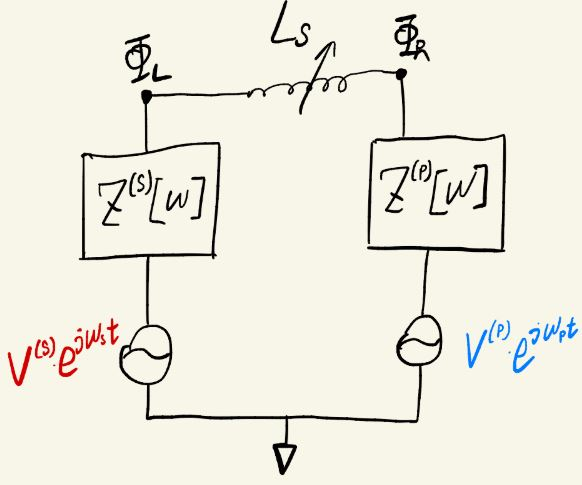
\includegraphics[width=7cm]{figures/circuit_2}
\caption
{\label{fig:circuit_2} Thevenin equivalent circuit}
\end{figure}

(Note that the relation between Thevenin voltage source $V^{(s/p)}$ and actual voltage at end of transmission line has to be simulated as well. )

For resonance parametric amplification, besides the pumpistor (acting like a negative resistance), we also need a mode around signal frequency. This section discusses how to guarantee a mode with well-defined frequency and SNAIL participation when designing external coupling network. 

When talking about resonance condition, let's first keep only the linear part of \eq{eq:It}: 

\begin{equation}\label{eq:LJ}
I(t) = I_c c_2 \tilde{\varphi} = 
\frac{\Phi_L(t) - \Phi_R(t) }{L_S} - M\phi_0\varphi_\min/L_S
\end{equation}

At the same time, the signal port network can be characterized by input impedance $Z^{(s)}$ (with the other port 50 $\Omega$ loaded), resulting in linear response between current $I$ and node voltage $V_L = \dot{\Phi}_L$: 
\begin{equation}\label{eq:LL}
	V_L(t) = - \integral{Z^{(s)}(t-\tau) I(\tau)}{\tau}{}{}
\end{equation}
and similarly for the right hand side: 
\begin{equation}\label{eq:RR}
	V_R(t) = \integral{Z^{(p)}(t-\tau) I(\tau)}{\tau}{}{}
\end{equation}

Laplace transform on \eq{eq:LL} and \ref{eq:RR}, as well as \eq{eq:LJ}, we get: 
\begin{equation}\label{eq:Is}
\begin{aligned}
I[s] &= \frac{\Phi_L[s] - \Phi_R[s] }{L_S}\\
-s \Phi_L[s] &= Z^{(s)}[s] I[s] \\
s \Phi_R[s] &= Z^{(p)}[s] I[s]
\end{aligned}
\end{equation}

or written equivalently:

\begin{equation}
\(
\begin{matrix}
1 & \frac{s}{Z^{(s)}} & 0 \\
1 & 0 & -\frac{s}{Z^{(p)}} \\
1 & -1/L_S & 1/L_S
\end{matrix}
\)	
\(
\begin{matrix}
I\\
\Phi_L\\
\Phi_R
\end{matrix}
\)
 = 0
\end{equation}

Existance of non-trivial solutions requires: 
\begin{equation}
	Z^{(s)}[s] + Z^{(p)}[s] =  - s L_S
\end{equation}

If we write $s = - \kappa/2 + j \omega$: 
\begin{align}
	\Im{Z^{(s)}[-\kappa/2 + j \omega]} + \Im{Z^{(p)}[-\kappa/2 + j \omega]} &=  - \omega L_S \label{eq:R1}\\
	\Re{Z^{(s)}[-\kappa/2 + j \omega]} + \Re{Z^{(p)}[-\kappa/2 + j \omega]} &=  \frac{\kappa}{2} L_S  \label{eq:R2}
\end{align}
Assuming a set of $\{\omega_k\}$ and $\{\kappa_k\}$ that satisfy these conditions, solution to the system will be in the form of linear combination of eigenmodes: 
\begin{equation}
	I(t) = \sum_k I_{\omega_k} \exp{- \frac{\kappa_k}{2} t} \exp{j\omega_k t}
\end{equation}
with $\omega_k$ being frequency of the k-th eigenmode, and $\kappa_k/2$ being amplitude damping rate of that mode (because we usually define $\kappa$ as energy damping rate). 

To design an SPA mode with arbitrary coupling networks, imaginary (reactive) parts of input impedance $Z^{(s)}$ and $Z^{(p)}$ has to satisfy requirement \ref{eq:R1} at desired mode frequency $\omega_a$. And reasonable $\kappa$ for this mode has to be achieved by real part of $Z^{(s)}$ (since $\Re{Z^{(p)}}$ should be close to 0 to prevent signal leakage from pump port). Note that SNAIL expansion parameter $c_2$ is dependent on external flux bias. As $L_S$ varies with flux, so does the $\omega$ that satisfies \eq{eq:R1}, thus tunes the mode frequency. For degenerate amplification, no other modes should exist within the frequency range of interest. 

(Extract SNAIL inductance participation from slope of imaginary part of input impedance)

We can always get \textbf{energy participation} of a component from field simulation. And what we usually do is assuming the SNAIL is a lumped inductive element (no E field energy stored in it), then \textbf{inductance participation} is always twice the energy perticipation. 

Here I propose an easier way to do so by extracting SNAIL \textbf{inductance participation} in the mode, which lay a requirement for the input impedances "apriori" before a full field simulation. This would be easier than "run HFSS and change paramters" especially when we want to optimize multiple things iteratively. 

We can generally define total admittance of the loop $Y_\sys[\omega] = \(Z^{(s)}[\omega] + Z^{(p)}[\omega] + j \omega L_S\)^{-1}$. 

An assumption I make is that behaviour of $Y_\sys[\omega]$ near $\omega_a$ (for whatever frequency my signal could lie) can be modeled for by a simple RLC. (This assumption is much weaker than Foster theorem: I'm only talking about one mode.)

\begin{figure}[htb]
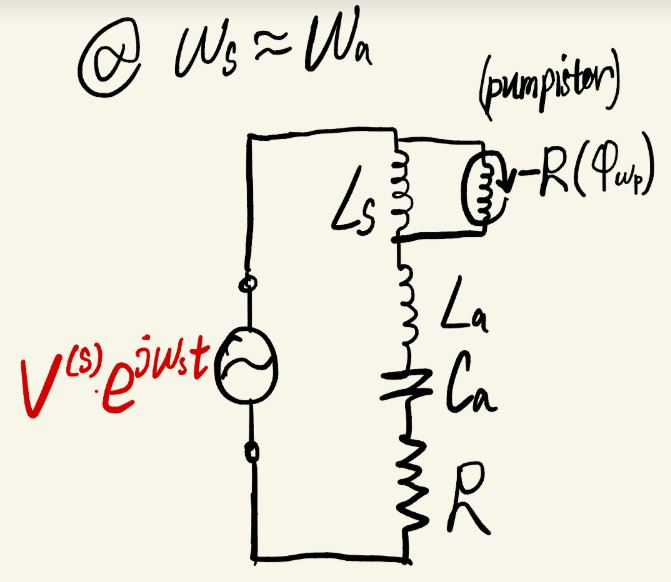
\includegraphics[width=6.5cm]{figures/circuit_3}
\caption
{\label{fig:circuit_3} Approximate circuit at $\omega_s \approx \omega_a$}
\end{figure}

The signal Thevenin voltage source $V^{(s)}$ sees the whole system as $Y_\sys[\omega_s]$, that responds exactly the same (for near resonance $\omega_s$) as a series RLC. 

The RLC model should account for the mode frequency $\omega_a$, residual of $\Im{Y_\sys}$ at $\omega_a$, and energy damping rate $\kappa$ of the mode. (To account for amplification, we should put a pumpistor in parallel with $L_S$.) 

\par
\par
**How this model helps: 

Using this model, we can calculate equivalent $L_a$ and $C_a$ from the values and slopes of imaginary part of the two input impedances (from linear simulation). 
All later nonlinearity calculation can be easily done analytically, and all existing results from mode amplitude $a$ and $\ad$ language applies directly. 
Doesn't involve the simulated $Z[\omega]$ function in calculation, and doesn't need harmonic balance simulation. 

Note that 4-th and higher orders nonlinearity calculated from this circuit are different from Foster circuit BBQ. Following the current conservation argument in Appendix A of \cite{SPA}, we have to treat the nonlinear inductance in series with linear inductance, unlike in Foster circuit BBQ where nonlinearity is treated in parallel with linear part. Another way to interprate the reason why Foster BBQ break down for SPA is that SNAIL participation in higher modes are non-negligible, therefore renormalization from higher modes has to be accounted for. 






\section{Calculation: two-port SPA pump leakage}\label{appen:leakage}

...... Easy part, just get the relation between $\varphi_{\omega_p}$ and $V^{(p)}$, calculate how much power at end of pump port transmission line gives $\varphi_{\omega_p}$ we need. 

And convert (using signal port network simulation result) the current $I_{\omega_p}$ into power seen by signal port transmission line. 

I've assumed stiff pump, which means I didn't do full harmonic balance. Which is doable though, by writing the \eq{eq:IV} like relation at $\omega_p$ also, and solving the three self-consistently. 
(This will allow us to characterize pump depletion. But I personally don't want to do it this way. Filters have kind of complicated response over pump frequency range, and we'll have to use simulated $Z^{(p)}[\omega]$ in all calculations. That could result in less robustness in simulation result and larger deviation between simulation and experiment. Also, I think this is not directly related to the main point of this paper.)






% After getting $Z_\ZPF$ of the mode, we can quantize this mode and perform a strict QLE treatment to explain the coupling rate. 


% \begin{align}
% \dot{\Phi} &= \frac{Q}{C_a} \label{eq:Phidotdir} \\
% \dot{Q} &= -\frac{\Phi}{L_a} - \frac{1}{Z_C}(\dot{\Phi} - V_\in) \label{eq:Qdotdir}
% \end{align}
% where $V_\in(t)$ is drive voltage at the end of transimion line.

% Introducing annihilation/creation operator according to $\Phi = \Phi _\ZPF (a + \ad)$ and $Q =\ii Q_\ZPF (\ad - a)$, where:
% \begin{equation}
% \Phi_\ZPF = \sqrt{\frac{\hbar}{2} Z_\ZPF}, \qquad Q_\ZPF = \sqrt{\frac{\hbar}{2 Z_\ZPF}}
% \end{equation}

% and $Z_\ZPF = \sqrt{(L_S+L_a)/C_a}$. Then \eq{eq:Phidotdir} is equivalent to: 

% \begin{equation}\label{eq:a1}
% \dot{a} + \dot{a}^\dagger = \frac{\ii Q_\ZPF}{\Phi_\ZPF C_a} (\ad- a) = \ii \omega_a (\ad - a)
% \end{equation}





% We can decompose the Heisenberg picture operator $a(t)$ in Fourier space: 

% \begin{equation}\label{eq:aFT}
% a(t) = \frac{1}{2\pi} \integral{a[\omega] \exp{- \ii \omega t}}{\omega}{-\inf}{\inf}
% \end{equation}

% And \eq{eq:a1} in Fourier domain can be written as: 

% \begin{equation}\label{eq:a2}
% \ad[-\omega] = -\frac{\omega-\omega_a}{\omega+\omega_a} a[\omega]
% \end{equation}



% (Arbitrary coupling)

% Outgoing current from the system: 
% \begin{equation}
% \begin{aligned}
% I_\out(t) &= \frac{1}{2\pi}\integral{I_\out[\omega]\exp{j\omega t}}{\omega}{-\inf}{\inf} \\
% &= \frac{1}{2\pi}\integral{\left( j \omega \Phi_\ZPF (a[\omega] + \ad[-\omega]) - V_\in[\omega] \right) Y_\tot[\omega]\exp{j\omega t}}{\omega}{-\inf}{\inf}\\
% &= \frac{1}{2\pi}\integral{\left( j\frac{2\omega \omega_a}{\omega + \omega_a} \Phi_\ZPF a[\omega] - V_\in[\omega] \right) Y_\tot[\omega]\exp{j\omega t}}{\omega}{-\inf}{\inf}
% \end{aligned}
% \end{equation}


% The total admittance seen by the system is: 
% \begin{equation}\label{eq:Ytot}
% Y_\tot[\omega] = \frac{1}{Z[\omega]+Z_C}
% \end{equation}


% And the Quantum Langevin Equations under arbitrary coupling, which are the generalized case of $\eq{eq:Phidotdir}$ and $\eq{eq:Qdotdir}$, should be written as: 

% \begin{align}
% \dot{\Phi} &= \frac{Q}{C_a} \label{eq:Phidot} \\
% \dot{Q} &= -\frac{\Phi}{L_a} - I_\out(t) \label{eq:Qdot}\\
% I_\out[\omega] &= \left(j \omega \Phi[\omega] - V_\in[\omega]  \right) Y_\tot[\omega] \label{eq:Iout}
% \end{align}

% where we notice that the EOM of $\Phi$ doesn't change, so \eq{eq:a1} still stands. And \eq{eq:Qdot} can be written into: 

% \begin{equation}\label{eq:a3}
% \ii (\dot{a}^\dagger - \dot{a}) = -\omega_a (\ad + a) - \frac{1}{Q_\ZPF} I_\out
% \end{equation}


% Using \eq{eq:aFT} and \eq{eq:a2} we can obtain: 

% % \begin{equation}\label{eq:FT1}
% % \begin{aligned}
% % - \ii (\dot{a}^\dagger - \dot{a}) &= \frac{1}{2\pi}\integral{\left(\omega a[\omega] \exp{-\ii \omega t} + \omega a^\dagger[\omega] \exp{\ii \omega t}\right)}{\omega}{-\inf}{\inf} \\
% %   &= \frac{1}{2\pi}\integral{\omega ( a[\omega] - a^\dagger[- \omega] )\exp{- \ii \omega t}}{\omega}{-\inf}{\inf} \\
% %   &= \frac{1}{2\pi}\integral{ \frac{2\omega^2}{\omega + \omega_a} a[\omega] \exp{j \omega t}}{\omega}{-\inf}{\inf}
% % \end{aligned}
% % \end{equation}

% \begin{equation}
% \begin{aligned}
% \dot{a}^\dagger + \dot{a} &= \frac{1}{2\pi}\integral{\left(a[\omega] \exp{-\ii \omega t} + \ad[\omega] \exp{\ii \omega t}\right)}{\omega}{-\inf}{\inf} \\
% &= \frac{1}{2\pi}\integral{( a[\omega] + \ad[- \omega] )\exp{- \ii \omega t}}{\omega}{-\inf}{\inf} \\
% &= \frac{1}{2\pi}\integral{ \frac{2\omega_a}{\omega + \omega_a} a[\omega] \exp{j \omega t}}{\omega}{-\inf}{\inf}
% \end{aligned}
% \end{equation}


% And using \eq{eq:Iout}, we can write down the last term in \eq{eq:a3} from inverse-Fourier transform: 
% \begin{equation}
% \begin{aligned}
% I_\out(t) &= \frac{1}{2\pi}\integral{I_\out[\omega]\exp{j\omega t}}{\omega}{-\inf}{\inf} \\
% &= \frac{1}{2\pi}\integral{\left( j \omega \Phi_\ZPF (a[\omega] + \ad[-\omega]) - V_\in[\omega] \right) Y_\tot[\omega]\exp{j\omega t}}{\omega}{-\inf}{\inf}\\
% &= \frac{1}{2\pi}\integral{\left( j\frac{2\omega \omega_a}{\omega + \omega_a} \Phi_\ZPF a[\omega] - V_\in[\omega] \right) Y_\tot[\omega]\exp{j\omega t}}{\omega}{-\inf}{\inf}
% \end{aligned}
% \end{equation}


% Now we can finally rewrite the Quantum Langevin Equation \eq{eq:a3} in Fourier domain: 

% \begin{equation}
% \frac{2\omega^2}{\omega + \omega_a} a[\omega] =\frac{2\omega_a^2}{\omega + \omega_a}a[\omega] + \left( j\frac{2\omega \omega_a}{\omega + \omega_a} \Phi_\ZPF a[\omega] - V_\in[\omega] \right) \frac{Y_\tot[\omega]}{Q_\ZPF}
% \end{equation}

% \begin{equation}\label{eq:QLE}
% \left( \omega - \omega_a - j \frac{\omega \omega_a}{\omega + \omega_a} Z_\ZPF Y_\tot[\omega]\right) a[\omega] = - \frac{Y_\tot[\omega]}{2Q_\ZPF} V_\in[\omega]
% \end{equation}

% We can write \eq{eq:QLE} as: 
% \begin{equation}
% 	\left(\Delta[\omega] + \ii \frac{\kappa[\omega]}{2}\right)a[\omega] = -u[\omega]
% \end{equation}


% detuning: 
% \begin{equation}
% 	\Delta[\omega] = \omega - \omega_a - \frac{\omega \omega_a}{\omega + \omega_a} Z_\ZPF \Im Y_\tot[\omega]
% \end{equation}

% kappa for arbitrary coupling:
% \begin{equation}\label{eq:kappa}
% 	\kappa[\omega] = \frac{2 \omega_a \omega}{\omega_a + \omega} Z_\mathrm{ZPF} \Re Y_\tot[\omega]
% \end{equation}


% For an resonance mode $\omega_a = 1 / \sqrt{L_a C_a}$    ,    $Z_\mathrm{ZPF} = 1/\omega_a C_a$

% For direct coupling:$Y = 1/Z_C$ ,  $\kappa_d = 1/C_a Z_C$.

% For capacitive coupling: 
% \begin{equation}\label{eq:Y_c}
% Y_\tot[\omega] = \frac{1}{Z_C + \frac{1}{j \omega C_c}} \approx j \omega C_c (1-j \omega C_c Z_C)
% \end{equation}

% Therefore: 
% \begin{equation}\label{eq:kappa_c}
% \kappa_c = \frac{Z_C}{L_a}\frac{C_c^2}{C_a^2}=Z_C \omega_a^2\frac{C_c^2}{C_a}
% \end{equation}





\bibliography{}

\end{document}